%% BioMed_Central_Tex_Template_v1.06
%%                                      %
%  bmc_article.tex            ver: 1.06 %
%                                       %

%%IMPORTANT: do not delete the first line of this template
%%It must be present to enable the BMC Submission system to
%%recognise this template!!

%%%%%%%%%%%%%%%%%%%%%%%%%%%%%%%%%%%%%%%%%
%%                                     %%
%%  LaTeX template for BioMed Central  %%
%%     journal article submissions     %%
%%                                     %%
%%          <8 June 2012>              %%
%%                                     %%
%%                                     %%
%%%%%%%%%%%%%%%%%%%%%%%%%%%%%%%%%%%%%%%%%


%%%%%%%%%%%%%%%%%%%%%%%%%%%%%%%%%%%%%%%%%%%%%%%%%%%%%%%%%%%%%%%%%%%%%
%%                                                                 %%
%% For instructions on how to fill out this Tex template           %%
%% document please refer to Readme.html and the instructions for   %%
%% authors page on the biomed central website                      %%
%% http://www.biomedcentral.com/info/authors/                      %%
%%                                                                 %%
%% Please do not use \input{...} to include other tex files.       %%
%% Submit your LaTeX manuscript as one .tex document.              %%
%%                                                                 %%
%% All additional Figures and files should be attached             %%
%% separately and not embedded in the \TeX\ document itself.       %%
%%                                                                 %%
%% BioMed Central currently use the MikTex distribution of         %%
%% TeX for Windows) of TeX and LaTeX.  This is available from      %%
%% http://www.miktex.org                                           %%
%%                                                                 %%
%%%%%%%%%%%%%%%%%%%%%%%%%%%%%%%%%%%%%%%%%%%%%%%%%%%%%%%%%%%%%%%%%%%%%

%%% additional documentclass options:
%  [doublespacing]
%  [linenumbers]   - put the line numbers on margins

%%% loading packages, author definitions

%\documentclass[twocolumn]{bmcart}% uncomment this for twocolumn layout and comment line below
% \documentclass[linenumbers, doublespacing]{bmcart}
\documentclass{bmcart}

%%% Load packages
\usepackage{amsthm,amsmath}
\RequirePackage{natbib}
% \RequirePackage[authoryear]{natbib}% uncomment this for author-year bibliography
\RequirePackage{hyperref}
% \usepackage[utf8]{inputenc} %unicode support
%\usepackage[applemac]{inputenc} %applemac support if unicode package fails
%\usepackage[latin1]{inputenc} %UNIX support if unicode package fails
\usepackage{lmodern}% http://ctan.org/pkg/lm
\usepackage{subcaption} %for subfigures
\usepackage{graphicx} %graphics support to specify path
\usepackage{csvsimple} %insert tables using .csv files
\usepackage{caption}

%%%%%%%%%%%%%%%%%%%%%%%%%%%%%%%%%%%%%%%%%%%%%%%%%
%%                                             %%
%%  If you wish to display your graphics for   %%
%%  your own use using includegraphic or       %%
%%  includegraphics, then comment out the      %%
%%  following two lines of code.               %%
%%  NB: These line *must* be included when     %%
%%  submitting to BMC.                         %%
%%  All Figure files must be submitted as      %%
%%  separate graphics through the BMC          %%
%%  submission process, not included in the    %%
%%  submitted article.                         %%
%%                                             %%
%%%%%%%%%%%%%%%%%%%%%%%%%%%%%%%%%%%%%%%%%%%%%%%%%


% \def\includegraphic{}
% \def\includegraphics{}

\graphicspath {{figures/}}

%%% Put your definitions there:
\startlocaldefs
\endlocaldefs


%%% Begin ...
\begin{document}

%%% Start of article front matter
\begin{frontmatter}

\begin{fmbox}
\dochead{Methodology}

%%%%%%%%%%%%%%%%%%%%%%%%%%%%%%%%%%%%%%%%%%%%%%
%%                                          %%
%% Enter the title of your article here     %%
%%                                          %%
%%%%%%%%%%%%%%%%%%%%%%%%%%%%%%%%%%%%%%%%%%%%%%

\title{Tissue Enrichment Analysis: TEA}

%%%%%%%%%%%%%%%%%%%%%%%%%%%%%%%%%%%%%%%%%%%%%%
%%                                          %%
%% Enter the authors here                   %%
%%                                          %%
%% Specify information, if available,       %%
%% in the form:                             %%
%%   <key>={<id1>,<id2>}                    %%
%%   <key>=                                 %%
%% Comment or delete the keys which are     %%
%% not used. Repeat \author command as much %%
%% as required.                             %%
%%                                          %%
%%%%%%%%%%%%%%%%%%%%%%%%%%%%%%%%%%%%%%%%%%%%%%

\author[
   addressref={aff1},                   % id's of addresses, e.g. {aff1,aff2}
   email={dangeles@caltech.edu}   % email address
]{\inits{DA}\fnm{David} \snm{Angeles-Albores}}
\author[
   addressref={aff2},                   % id's of addresses, e.g. {aff1,aff2}
   email={raymond@caltech.edu}   % email address
]{\inits{RYL}\fnm{Raymond Y} \snm{Lee}}
\author[
   addressref={aff2},                   % id's of addresses, e.g. {aff1,aff2}
   email={azurebrd@caltech.edu}   % email address
]{\inits{JC}\fnm{Juancarlos} \snm{Chan}}
\author[
   addressref={aff1, aff3},
   corref={aff1},
   email={pws@caltech.edu}
]{\inits{PWS}\fnm{Paul W} \snm{Sternberg}}


%%%%%%%%%%%%%%%%%%%%%%%%%%%%%%%%%%%%%%%%%%%%%%
%%                                          %%
%% Enter the authors' addresses here        %%
%%                                          %%
%% Repeat \address commands as much as      %%
%% required.                                %%
%%                                          %%
%%%%%%%%%%%%%%%%%%%%%%%%%%%%%%%%%%%%%%%%%%%%%%

\address[id=aff1]{%                           % unique id
  \orgname{California Institute of Technology, Division of Biology and Biological Engineering}, % university, etc
  \street{1200 E California Blvd},                     %
  \postcode{91125},                               % post or zip code
  \city{Pasadena},                              % city
  \cny{US}                                    % country
}

\address[id=aff3]{%                           % unique id
  \orgname{HHMI}, % university, etc
}

% raymond's address?
\address[id=aff2]{%
  \orgname{California Institute of Technology},
  \street{1200 E California Blvd},                     %
  \postcode{91125},                                % post or zip code
  \city{Pasadena},                              % city
  \cny{US}                                    % country
}

%%%%%%%%%%%%%%%%%%%%%%%%%%%%%%%%%%%%%%%%%%%%%%
%%                                          %%
%% Enter short notes here                   %%
%%                                          %%
%% Short notes will be after addresses      %%
%% on first page.                           %%
%%                                          %%
%%%%%%%%%%%%%%%%%%%%%%%%%%%%%%%%%%%%%%%%%%%%%%


\end{fmbox}% comment this for two column layout

%%%%%%%%%%%%%%%%%%%%%%%%%%%%%%%%%%%%%%%%%%%%%%
%%                                          %%
%% The Abstract begins here                 %%
%%                                          %%
%% Please refer to the Instructions for     %%
%% authors on http://www.biomedcentral.com  %%
%% and include the section headings         %%
%% accordingly for your article type.       %%
%%                                          %%
%%%%%%%%%%%%%%%%%%%%%%%%%%%%%%%%%%%%%%%%%%%%%%

\begin{abstractbox}

\begin{abstract} % abstract
\parttitle{Background} %if any
Over the last ten years, there has been an explosive development in tools
capable of measuring gene expression. These tools generate a large number
of gene targets, but understanding these datasets, and forming hypotheses
based on them remains challenging. One way to analyze these datasets is to
associate ontologies, which are controlled, hierarchical, descriptive vocabularies
with genes and to look for enrichment of specific terms. Although gene ontology
(GO) is available for \emph{C. elegans}, this ontology does not include
anatomy or physiology information.
\parttitle{Results} %if any
We have developed an enrichment analysis tool for the \emph{C. elegans} tissue
ontology, is available on the web via WormBase and is available for download 
using Python's standard pip installer. In order to cut down on verbosity, we
have come up with three straightforward filtering criteria that slim the ontology
by almost tenfold. 
\parttitle{Conclusions} %if any
Our Tissue Enrichment Analysis (TEA), which can be found at www.wormbase.org/tea, 
uses a standard hypergeometric function to test a slimmed-down \emph{C. elegans} tissue 
ontology and provides users with a text and graphic representation of the results. 
\end{abstract}

%%%%%%%%%%%%%%%%%%%%%%%%%%%%%%%%%%%%%%%%%%%%%%
%%                                          %%
%% The keywords begin here                  %%
%%                                          %%
%% Put each keyword in separate \kwd{}.     %%
%%                                          %%
%%%%%%%%%%%%%%%%%%%%%%%%%%%%%%%%%%%%%%%%%%%%%%

\begin{keyword}
\kwd{Gene Ontology}
\kwd{Tissue Ontology}
\kwd{WormBase}
\kwd{RNA-seq}
\kwd{High-throughput biology}
\end{keyword}

% MSC classifications codes, if any
%\begin{keyword}[class=AMS]
%\kwd[Primary ]{}
%\kwd{}
%\kwd[; secondary ]{}
%\end{keyword}

\end{abstractbox}
%
%\end{fmbox}% uncomment this for twcolumn layout

\end{frontmatter}

%%%%%%%%%%%%%%%%%%%%%%%%%%%%%%%%%%%%%%%%%%%%%%
%%                                          %%
%% The Main Body begins here                %%
%%                                          %%
%% Please refer to the instructions for     %%
%% authors on:                              %%
%% http://www.biomedcentral.com/info/authors%%
%% and include the section headings         %%
%% accordingly for your article type.       %%
%%                                          %%
%% See the Results and Discussion section   %%
%% for details on how to create sub-sections%%
%%                                          %%
%% use  \cite{...} to cite references        %%
%%   \cite{koon} and                         %%
%%   \cite{oreg,khar,zvai,xjon,schn,pond}    %%
%%  \nocite{smith,marg,hunn,advi,koha,mouse}%%
%%                                          %%
%%%%%%%%%%%%%%%%%%%%%%%%%%%%%%%%%%%%%%%%%%%%%%

%%%%%%%%%%%%%%%%%%%%%%%%% start of article main body
% <put your article body there>

%%%%%%%%%%%%%%%%
%% Background %%
%%
\section*{Background}
	RNA-seq and other high-throughput methods in biology have the ability to identify thousands of genes that are altered between conditions. These genes are often correlated in their biological characteristics or functions, but identifying these functions remains challenging. To interpret these long lists of genes, biologists need to abstract genes into fewer terms that are biologically relevant to form hypotheses about what is happening in the data. One such abstraction method relies on Gene Ontology (GO). GO provides a controlled set of hierarchically ordered terms in the form of an directed acyclic graph  \cite{TheGeneOntologyConsortium2000, Ontology2009, TheGeneOntologyConsortium2015} that provide detailed information about the molecular, cellular or biochemical functions of the gene among others. For a given gene list, certain software programs can query whether a particular gene is enriched  \cite{Mi2009, McLean2010, Huang2009}. One area of biological significance that GO does not include is physiology and anatomy. One way to address this shortcoming is to generate a `tissue ontology' that provides a complete anatomical description for an organism or sets of organisms, such as `tissue', `organ' or `neuronal cell', for example. Such a tissue ontology has been developed previously \cite{Lee2003}.  The C. elegans  database, Wormbase \cite{Harris2014}, maintains a carefully curated list of gene expression data from GFP-reporters. 
	Here we provide a new framework that analyses user-input list for enrichment of specific tissues. We believe that tissues are physiologically relevant units with broad, relatively well-understood functionalities amenable to hypothesis formation. As such, we believe that identification of tissues is likely to provide researchers with enough information to be able to form hypotheses about the physiological responses of an organism to a specified condition. 
	
	Another problem frequently associated with GO analaysis is that it is often difficult to interpret due to the large number of terms associated with a given gene. There exist a number of GO analytic tools for use by the community but a shared complaint for many programs is the very large number of GO terms that are significantly associated with any given gene list.  A common tool for GO analysis, DAVID, clusters terms into broad categories that are amenable to exploration by researchers  \cite{Huang2007}, whereas PANTHER, a different software package  \cite{Mi2009, Mi2013}, attempts to solve this issue by employing a manually reduced ontology, GOslim (pers. comm. H. Yu and P. Thomas).
	
	To prevent our tool from suffering from the same drawbacks, we have cut down on result verbosity by filtering the ontology by using a small set of well-defined criteria to remove terms that do not contribute extra information. To our knowledge, such filtering has never been performed in an algorithmic fashion for an ontology before---indeed, tools such as DAVID do not employ term trimming \emph{a priori} of testing, but rather fuzzy clustering \emph{post} testing to reduce the number of ontology terms. We believe our trimming methodology strikes a good balance between detailed tissue calling and conservative testing.	

	Our tool is available within WormBase and provides users with a text-based file of the enrichment results as well as a simple and clear graph of the results that exhibit the largest fold-change enrichment.

\section*{Results}
\subsection*{Generating a Useful Dictionary}
\subsubsection*{Reducing term redundancy through a similarity metric}
As a first step to generate our tissue enrichment software, we wished to select tissue terms that were reasonably well-annotated, yet specific enough to provide insight and not redundant with other terms. We also wanted to avoid testing tissues at levels where redundancy becomes problematic. For example, several left and right neurons have at least 25 annotating genes and we may want to include them for enrichment testing. However, many left/right neuronal pairs (which are sisters in the ontology) have almost identical annotations, with at most one or two gene differences between them. We reasoned that when two tissues have almost identical annotations, we cannot have statistical confidence in differentiating between them. As a result, testing these sister tissues provides no additional information compared with testing only the parent node to these sisters. We refer to such sisters as `redundant'. To identify redundancy, we defined a similarity metric (see \emph{Methods} section and Figure~\ref{fig:simdiagram}). Our similarity metric can be used to identify sisters that have very high similarity between them; alternatively, redundant sisters could be identified if a single sister had a very high similarity score. We referred to these two scoring criteria as `avg' and `any' respectively. 

\subsubsection*{Terminal branch terms and parent terms can be safely removed in an algorithmic fashion }
Another problem arises from the fact that the tissue ontology is scarcely populated at this point in time. Many nodes have 0-10 annotations, which we consider too few to accurately test. To solve this issue, we implemented a straightforward trimming algorithm. For a given terminal node, we test whether the node has more than a threshold number of annotations. If it does not, the node is removed. The next node in the branch is tested and removed recursively until a node which satisfies the condition is found. At that point, no more nodes can be removed from that branch. This is guaranteed by the structure of the ontology: Parent nodes inherit all of the annotations of all of their descendants, so the number of annotating terms monotonically increases with increasing term hierarchy (see Figure~\ref{fig:trim_ends}). In this way, we ensure that our term dictionary includes only those tissues that are considered sufficiently well annotated for statistical purposes.

	Finally, we also wanted to remove as many terms as possible from the dictionary with the goals of reducing covariance between terms, decreasing multiple testing and removing as many non-informative terms as possible. Decreasing covariance between terms is important because we employ a frequentist approach that assumes all terms are independent. Large covariation coefficients between some terms means that if one of these tissues tests significant, the other terms are much more likely to pass significance testing as well. This makes adequate correction for false positive rates considerably more difficult. Moreover, from a data analysis perspective, we reasoned that, for any parent node, if all its daughters were selected for testing, there was no additional benefit to test the parent. In other words, if all the daughter nodes are tested, there is little additional information to be gained by including the parent node.  To address this issue we removed parent nodes from the analysis if all their daughter nodes passed the annotation threshold (see Figure~\ref{fig:trim_roots}).

\subsubsection*{Filtering greatly reduces the number of nodes used for analysis}
	By itself, each of these filters can reduce the number of nodes employed for analysis. Notably, these filters are not all commutative: while trimming and redundancy filtering are commutative, applying the ceiling filter is not commutative with either the trimming or the redundancy filter. If the ceiling filter is  applied before any other filter, only terminal nodes will remain, since all the parents have complete daughter sets. Since terminal nodes are the most poorly annotated, after applying the remaining filters very few nodes will be left behind if any. On the other hand, applying the ceiling operator after trimming and redundancy filtering  will result in greater numbers of nodes. We always applied the ceiling at the end. For validation (see below) we made a number of different dictionaries. The original ontology has 1675 terms with more than 5 gene annotations. After filtering, dictionary sizes ranged from 21 to a maximum of 400 terms, which shows the number of terms in a scarcely annotated ontology can be reduced by tenfold by application of a few simple filters (see Table ~\ref{tab:DictionarySpecs}). These filters were used to compile a static dictionary that we employ for all analyses.

\subsection*{Tissue enrichment testing via a hypergeometric model}
	Having built a static dictionary, we generated a Python script that implements a significance testing algorithm based on the hypergeometric model. Briefly, the hypergeometric model assumes the existence of an urn with a pre-determined number of balls inside it. The balls can be painted one of several colors. The hypergeometric model provides an answer to the question: If an individual removes $N$ balls, what is the probability of observing $n_i$ balls of color $i$, if the balls are selected without replacement? Mathematically, this is expressed as:
\begin{eqnarray}\label{hypergeometric}
	\mathrm{P}(n_i | N, m_i, M) = \frac{\dbinom{m_i}{n_i} \dbinom{M-m_i}{N - n_i}}{\dbinom{N}{n_i}}
\end{eqnarray}
	Here, $n_i$ is the number of balls of type $i$ drawn, $N$ is the total number of draws, $m_i$ is tissue $i$ and $M$ is the total number of balls in the urn. In our specific case, $M_i$ is equal to the total number of annotations in our dictionary. $N$ is found by taking the user-input list and removing any genes that are not in our annotation dictionary. The remaining genes are then associated with their annotation profiles---if a tissue is associated with $s$ tissues, it generates $s$ balls of $s$ colors. Our program counts the number of times each tissue appears in the user list, and calculates the probability of having withdrawn as many or more balls for each tissue in the user list. Due to the discrete nature of the hypergeometric distribution, this algorithm can generate artifacts when the list is small. To avoid spurious results, a tissue is never considered significant if there are no annotations for it in the user-provided list.

	Once the probability of drawing the labels has been quantified, we apply a standard FDR correction using a Benjamini-Hochberg step-up algorithm \cite{Benjamini1995}. Genes that have a q-value less than a given alpha are considered significant. Our default setting is to set the alpha threshold at 0.1, but users will be able to modify this value either in batch or in our web application. The program returns a text-based table showing the tissues that tested significant, along with their associated q-value, the expected number of hits for a list of that size, the observed number of hits and the enrichment fold change (observed hits / expected hits). Finally, the program can also return a bar chart of the enrichment fold change for the fifteen tissues with the lowest measured q-values.
	Our software is implemented in an easy to use GUI within WormBase. Users input a gene-list using any valid gene name for \emph{C. elegans}. These names are processed into standard WBIDs and the result is displayed in the same window in an easy to read format containing all the relevant information, and a graph of the results is also displayed (see Figure ~\ref{fig:GUIresults}).

\subsection*{Validation of the algorithm and parameter selection}
	We wanted to select a dictionary which included enough terms to be specific beyond the largest C. elegans tissues, yet would minimize the number of spurious results and which had a good dynamic range in terms of enrichment fold-change. Selection of a dictionary based only on minimization of spurious results would result in a dictionary with a large number of annotations per tissue, and would therefore include only the major tissues. On the other hand, selecting a dictionary that can detect smaller tissues will bias us towards tissues with lesser annotations. To our knowledge there is no good method for assessing false-positive or false-negative results for annotations.To help us select an appropriate dictionary and validate our tool, we found a set of 30 gold standards based on microarray and RNA-seq literature which are believed to be enriched in specific tissues \cite{Gaudet2004a, Spencer2011, Cinar2005, Watson2008a, Pauli2006, Portman2004, Fox2007, Smith2010}. Some of these studies have been used to annotate gene expression, and so they did not constitute an independent testing set. To correct this flaw, we built a clean dictionary that specifically excluded all annotation evidence that came from these studies.

	As a first attempt to select a good dictionary, we generated all the possible combinations of dictionaries with minimal annotations of 10, 25, 50 and 100 genes and similarity cutoffs of 0.9, 0.95 and 1, using `avg' or `any' thresholding criteria for the latter (see Table ~\ref{tab:DictionarySpecs}). For these dictionaries, the number of tissues tested ranged from 21 to 460. The number of tissues was inversely correlated to the minimum annotation, as expected, and was largely insensitive to the redundancy threshold, at least in the range we explored (0.9-1). Next, we analyzed all 30 datasets using each dictionary. Because of the large number of results, instead of analyzing each set of terms individually, we pooled all results for a given dictionary into histograms. When we analyzed the distribution of significant q-values for the dictionaries, we found that the similarity threshold mattered relatively little for any dictionary. We also noticed that the `any' thresholding method resulted in tighter histograms with a mode closer to 0. For this reason, we chose the `any' method for dictionary generation. The average q-value increased with decreasing annotation cut-off (see Figure~\ref{fig:qvals}), which reflects the decreasing statistical power associated with fewer annotations per term, but we remained agnostic as to how significant the trade-off between power and term specificity is. Based on these observations, we ruled out the dictionary with the 100 gene annotation cut-off: it had the fewest terms and its q-values were not low enough to compensate the trade-off in specificity.

%dictionaries that work well
To select between dictionaries generated between 50, 33 and 25 annotation cut-offs, and also to ensure the terms that are selected as enriched by our algorithm are reasonable, we looked in detail at the enrichment analysis results.
%Work well
Most results were highly comparable and in line with what was expected. For some sets, all dictionaries seemed to perform well. For example, in our `all neuron enriched sets'~ \cite{Spencer2011, Watson2008a} the results were an amalgamation of neuron related terms including mechanosensory neurons, thermosensitive neurons, interneurons, ganglions and male rays regardless of the dictionary used (see~\ref{fig:interagree}). On the other hand, when we looked at a gene set enriched for germline precursor expression in the embryo~ \cite{Spencer2011}, the dictionary with the 50 cutoff was only able to identify `oocyte WBbt:006797'; whereas the two smaller dictionaries were able to single out cells germline precursor cells ---at the 33-cutoff, our tool identified `Z2' and `Z3' as being five-fold enriched; whereas at the 25 gene-cutoff the terms `Psub4',`Psub3' and `Psub2' were identified in addition to `Z2' and `Z3'.
%Differences between dictionaries
We queried an embryonic stage intestine precursor geneset~ \cite{Spencer2011}. Notably, this gene set yielded no enrichment when using the 25 cutoff dictionary, nor when using the 50 cutoff dictionary. However, the 33 cutoff dictionary suggested, probably correctly, that the E lineage was heavily enriched in this set.
%Bad stuff.
Not all queries worked equally well. For example, a number of intestinal enriched genes sets~ \cite{Spencer2011, Pauli2006} were not enriched in intestine in any dictionary, but they were enriched for pharynx- and hypodermis-related terms. We were somewhat surprised that intestinal gene sets performed poorly, since the intestine is a relatively well-annotated tissue.
%Dictionary intra-agreement
We also assessed the internal agreement of our tool by using independent gene-sets that we expected to be enriched in the same tissues. We had two independent pan-neuronal sets~ \cite{Spencer2011, Watson2008a}; two independent PVD enriched sets~ \cite{Spencer2011, Smith2010}; two independent GABAergic gene sets~ \cite{Spencer2011, Cinar2005}; two independent pharyngeal gene sets~ \cite{Spencer2011, Gaudet2004a}; and two independent intestinal gene sets~ \cite{Spencer2011, Pauli2006}. Overall, the tool seems to have good internal agreement. On most sets, the same terms were enriched, although order was somewhat variable see ~\ref{fig:intragree}. However, most high-scoring terms were preserved between gene sets. The intestinal gene-sets and pharyngeal gene sets comparisons were exceptions, since at least one gene set was missing each for intestine and pharynx in every dictionary, so we didn't consider them as informative for assessing internal agreement.
 All comparisons can be found online in our Github repository (see Availability of data and materials). Overall, the dictionary generated by a 33 gene annotation cutoff with 0.95 redundancy threshold using the `any' criterion. seemed to perform well, with a good balance between specificity, verbosity and accuracy, so we selected this parameter set to generate our static dictionary.


\subsection*{A brief example}
We applied our tool to the RNA-seq datasets developed by Engelmann et al.  \cite{Engelmann2011} to gain further understanding of the biology underlying these datasets. Engelmann et al.  exposed young adult worms to 5 different pathogenic bacteria or fungi for 24 hours, after which mRNA was extracted from the worms for sequencing. We ran TEA on the genes Engelmann \emph{et al} identified as up- or down-regulated. Initially we noticed that genes that are down-regulated tend to be twice better annotated on average than genes that were up-regulated, suggesting that our understanding of the worm immune system is scarce, in spite of important advances made over the last decade. Strikingly, three out of the five samples showed enrichment of neuronal tissues or neuronal precursor tissues amongst the down-regulated genes (see \ref{fig:Dcon, fig:Hsp, fig:Smar}). A possible explanation for this might be that the infected worms are sick and the neurons are beginning to shut down; an alternative hypothesis would be that the worm is down-regulating specific neuronal pathways as a behavioural response against the pathogen. Indeed, several studies \cite{Meisel2014, Zhang2005} have provided evidence that \emph{C. elegans} uses chemosensory neurons to identify pathogens. Interestingly, one bacterium did not exhibit the same pattern of down-regulation of neuronal-associated genes. \emph{E. faecalis} showed increased expression of genes associated with neuronal tissues, hinting that \emph{E. faecalis} may have a different pathogenic profile. Up-regulated tissues, when detected, almost always included the hypodermis and excretory duct.
	Our results highlight the involvement of various \emph{C. elegans} neuronal tissues in pathogen defense and/or illness.

\section*{Discussion}
We have presented a tissue enrichment analysis tool that employs a standard hypergeometric model to test the \emph{C. elegans} tissue ontology. We have also presented the first, to our knowledge, ontology trimming algorithm. This algorithm, which is very easy to execute, places strong limits on the number of terms selected for testing. Due to the nature of all ontologies as hierarchical, acyclical graphs with term inheritance, term annotations are correlated along any given branch. This correlation reduces the benefits of including all terms for statistical analysis: for any given term along a branch, if that term passes significance, there is a high probability that many other terms along that branch will also pass significant. If the branch is enriched by random chance, error propagation along a branch means that many more false positives will follow. Thus, a researcher might be misled by the number of terms of correlated function and assign importance to this finding; the fact that the branching structure of GO amplifies false positive signals is a powerful argument for either reducing branch length or branch intracorrelation, or both. On the other hand, if a term is actually enriched, we argue that there is little benefit to presenting the user with additional terms along that branch. Instead, a user will benefit most from testing sparsely along the tree at a suitable specificity for hypothesis formation. Related terms of the same level should only be tested when there is sufficient annotation to differentiate, with statistical confidence, whether one term is enriched above the other. Our algorithm reduces branch length by identifying and removing nodes that are insufficiently annotated and parents that are likely to include sparse information.

Chikina \emph{et al}  \cite{Chikina2009} report a tissue enrichment model based on an SVM classifier that has been trained on microarray studies. SVM classifiers are powerful tools capable of great sensitivity, but they require continuous retraining as tissue expression data becomes more available. Moreover, classifiers require that data be rank-ordered by some metric, something which is not possible for some genome-wide studies. Our tool relies on an annotation dictionary that is continuously updated, does not require retraining and does not require ranked genes. To our knowledge, there are no other tissue ontology enrichment tools in \emph{C. elegans}, but similar projects exist for humans and zebrafish ~\cite{Lee2013, Prykhozhij2013}, highlighting the relevance of our tool for high-dimensionality biology.

We have tried hard to benchmark our tool well. However, our analysis suffers from the drawback that is very hard to benchmark negative controls. Even for our set of positive controls, the statistical analysis sometimes throws out unexpected results. For example, the embryonic germline precursor gene set had the term `AB' as the most enriched term in the dictionaries with cut off of 25 and 33. Is this an error, or does this hint at new biology? Although we were unable to determine false-positive and false-negative rates, we  do not believe this should deter scientists from using our tool. Rather, we encourage researchers to use our tool carefully as a guide, integrating evidence from multiple sources to inform the most likely hypotheses. As with any other tool based on statistical sampling, our analysis is most vulnerable to bias in the data collection stage. For example, we know that tissue expression reports are negatively biased against germline expression due to the difficulty associated with extrachromosomal array expression in that tissue. Support from the community will be crucial in correcting these flaws going forward; indeed, without the community reports of tissue expression this tool would not be possible.

\section*{Methods}
\subsection*{Filtering nodes}
\subsubsection*{Defining a Similarity Metric}
In order to identify redundant sisters, we defined the following similarity metric:
\begin{eqnarray}\label{similarity def}
	s_i = \frac{|g_i|}{|\bigcup_{i= 0}^k g_i|}
\end{eqnarray}
Where $s_i$ is the similarity for a tissue $i$ with $k$ sisters; $g_i$ refers to the set of tissues associated with tissue $i$ and $|g|$ refers to the cardinality of set $g$. For a given set of sisters, we called them redundant if they exceeded a given similarity threshold. We envisioned two possible criteria and built different dictionaries using each one. Under a threshold criteron `any' with parameter $S$ between $(0, 1)$, a given set of sisters $j$ was considered redundant if the condition
\begin{eqnarray}\label{any threshold}
	s_{i, j} > S
\end{eqnarray}
was true for any sister $i$ in set $j$. Under a threshold criterion `avg' with parameter $S$, a given set of sisters $j$ was considered redundant if the condition
\begin{eqnarray}\label{avg threshold}
	\mathrm{E}[s_i]_j > S
\end{eqnarray}
was true for the set of sisters $j$ (see Figure~\ref{fig:simdiagram}).

\subsubsection*{Implementation}
All scripts were written in Python. Our software relies on the Pandas, Numpy, Seaborn and SciPy modules to perform all statistical testing and data handling \cite{McKinney2011, VanDerWalt2011, Oliphant2007}.


\section*{Availability of data and materials}
Our web implementation is available at https://www.wormbase.org/tea. Our software can also be downloaded using Python's pip installer via the command

\texttt{pip install tissue\_enrichment\_tool}

Alternatively, our software is available for download at:

http://dangeles.github.io/TissueEnrichmentAnalysis

All benchmark gene sets, benchmarking code and Figures can also be found at the same address, under the `tests' folder.
%%%%%%%%%%%%%%%%%%%%%%%%%%%%%%%%%%%%%%%%%%%%%%
%%                                          %%
%% Backmatter begins here                   %%
%%                                          %%
%%%%%%%%%%%%%%%%%%%%%%%%%%%%%%%%%%%%%%%%%%%%%%

\begin{backmatter}

\section*{Competing interests}
 	The authors declare that they have no competing interests.
\section*{Author's contributions}
    DA and PWS conceived of the project; DA developed algorithm;
	RYL made intellectual contributions to the project; RYL and JC
	developed the web GUI.
\section*{Acknowledgements}
	We would like to acknowledge all members of the Sternberg
	lab for helpful discussion.
%%%%%%%%%%%%%%%%%%%%%%%%%%%%%%%%%%%%%%%%%%%%%%%%%%%%%%%%%%%%%
%%                  The Bibliography                       %%
%%                                                         %%
%%  Bmc_mathpys.bst  will be used to                       %%
%%  create a .BBL file for submission.                     %%
%%  After submission of the .TEX file,                     %%
%%  you will be prompted to submit your .BBL file.         %%
%%                                                         %%
%%                                                         %%
%%  Note that the displayed Bibliography will not          %%
%%  necessarily be rendered by Latex exactly as specified  %%
%%  in the online Instructions for Authors.                %%
%%                                                         %%
%%%%%%%%%%%%%%%%%%%%%%%%%%%%%%%%%%%%%%%%%%%%%%%%%%%%%%%%%%%%%

% if your bibliography is in bibtex format, use those commands:
\bibliographystyle{bmc-mathphys} % Style BST file (bmc-mathphys, vancouver, spbasic).
\bibliography{bmc_article}      % Bibliography file (usually '*.bib' )
% for author-year bibliography (bmc-mathphys or spbasic)
% a) write to bib file (bmc-mathphys only)
% @settings{label, options="nameyear"}
% b) uncomment next line
\nocite{label}

% or include bibliography directly:
% \begin{thebibliography}
% \bibitem{b1}
% \end{thebibliography}

%%%%%%%%%%%%%%%%%%%%%%%%%%%%%%%%%%%
%%                               %%
%% Figures                       %%
%%                               %%
%% NB: this is for captions and  %%
%% Titles. All graphics must be  %%
%% submitted separately and NOT  %%
%% included in the Tex document  %%
%%                               %%
%%%%%%%%%%%%%%%%%%%%%%%%%%%%%%%%%%%

%%
%% Do not use \listoffigures as most will included as separate files

\section*{Figures}

% Figures describing algorithm

\begin{figure}[h!]
  \begin{subfigure}[b]{0.3\textwidth}
    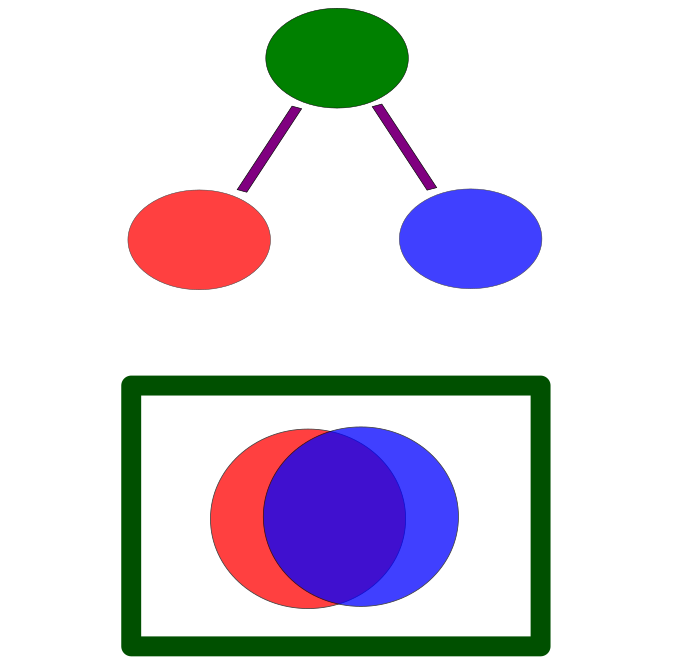
\includegraphics[width=\textwidth]{figures/RedundancyTrimmingOntogeny.png}
   	 	\caption{}
    \label{fig:simdiagram}
  \end{subfigure}
  %
  \begin{subfigure}[b]{0.3\textwidth}
    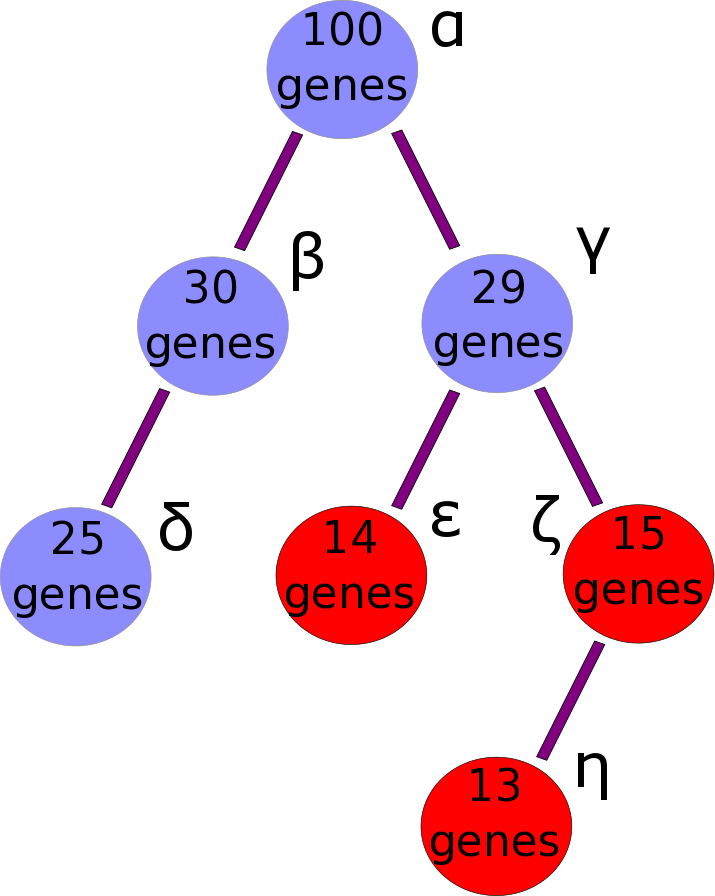
\includegraphics[width=\textwidth]{figures/FloorTrimmingOntogeny.png}
	      \caption{}
    \label{fig:trim_ends}
  \end{subfigure}
  \begin{subfigure}[b]{0.3\textwidth}
    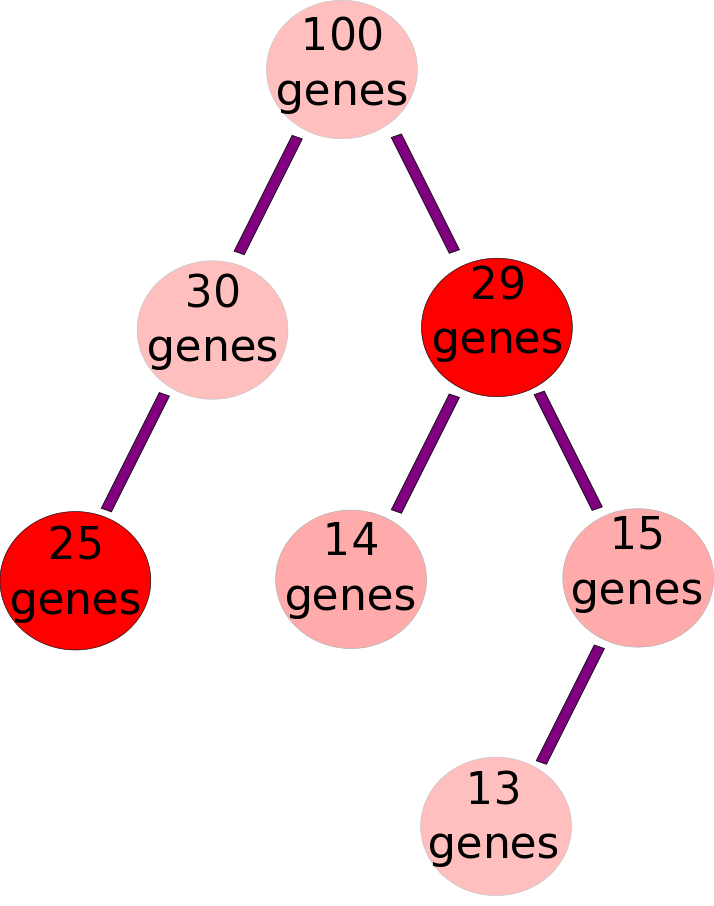
\includegraphics[width=\textwidth]{figures/CeilingTrimmingOntogeny.png}
    	\caption{}
    \label{fig:trim_roots}
  \end{subfigure}

  \captionsetup{width= 0.95\textwidth}
  \caption{
  	\csentence{Schematic representation of trimming filters for an acyclical ontology.}
    \csentence{\textbf{a)}} The parent node (green) contains at least as many annotations as the union of the two sisters. These two sisters share annotations extensively. Therefore they are too similar and should be removed.
	\csentence{\textbf{b)}} Nodes with less than a threshold number of genes are trimmed (light red) and discarded from the dictionary. Here, the example threshold is 25 genes.
	\csentence{\textbf{c)}} We trim parent nodes (light red) if all their daughter nodes have more than the threshold number of annotations.
  }
\end{figure}


%   \begin{figure}[h!]
%   \caption{\csentence{Schematic diagram of annotations for two sisters.}
%       The parent node (green) contains at least as many annotations as the union of the two sisters.
% 	  These two sisters share annotations extensively. Therefore they are too similar and should be removed.
% 	  }
% 	  % \label{fig:simdiagram}
%   \end{figure}
%
% \begin{figure}[h!]
%   \caption{\csentence{Schematic showing terminal node removal.}
%       Nodes with less than a threshold number of genes are trimmed (light red) and discarded from the dictionary. Here, the threshold is 25 genes.}
% 	  \label{fig:trim_ends}
%       \end{figure}
%
% \begin{figure}[h!]
%   \caption{\csentence{Schematic showing root node removal.}
%       We trim parent nodes (light red) if all their daughter nodes have more than the threshold number of annotations. Here, the threshold is 25 genes.}
% 	  \label{fig:trim_roots}
%       \end{figure}


%gui

\begin{figure}
  % \begin{subfigure}[b]{0.4\textwidth}
  %   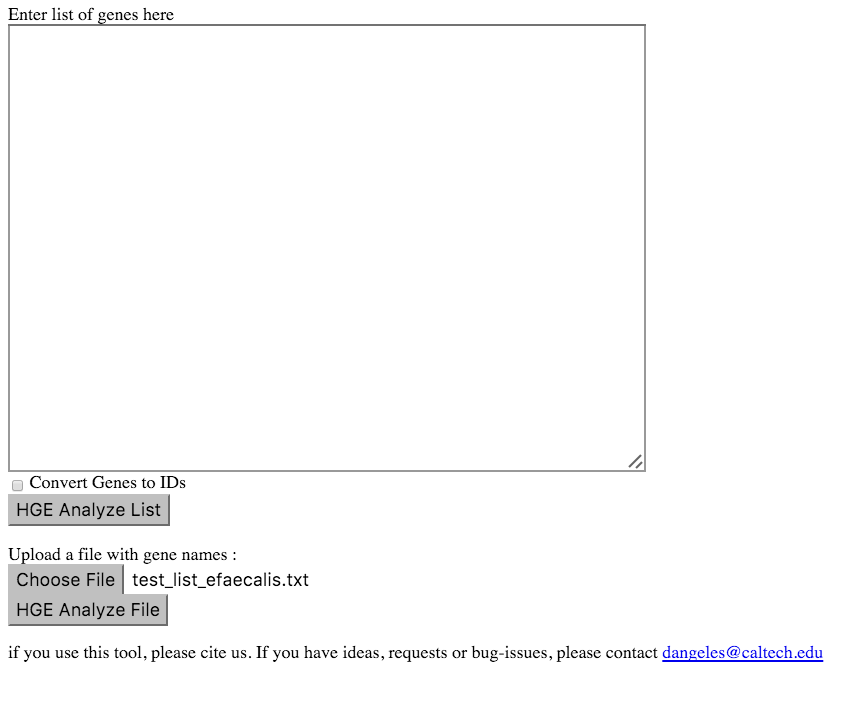
\includegraphics[width=\textwidth]{figures/gui.png}
  %   \caption{}
  %   \label{fig:GUI}
  % \end{subfigure}
  % %
  % \begin{subfigure}[b]{0.4\textwidth}
    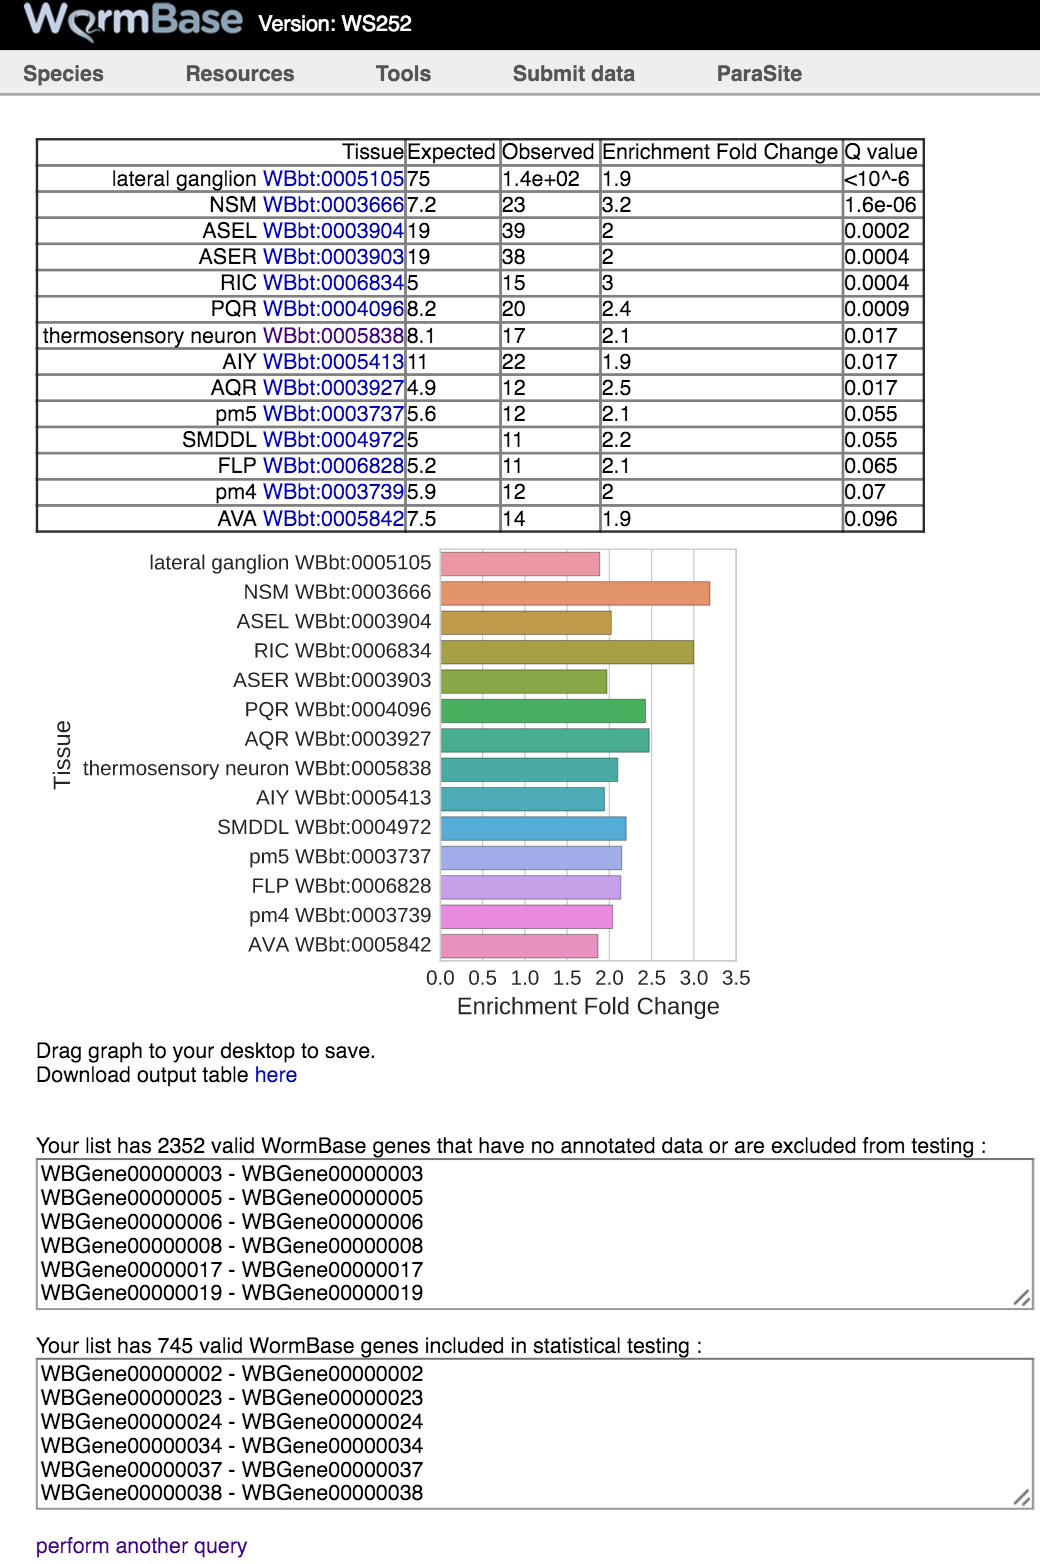
\includegraphics[width=\textwidth]{figures/guiresults.png}
    % \caption{}
  % \end{subfigure}
  \captionsetup{width= 0.95\textwidth}
  \caption{\csentence{Screenshot of results from the web GUI.}
  After inputting a gene-list, the user is provided with the results. 
  An HTML table is output with hyperlinks to the ontology terms. A 
  publication-ready graph is provided below, which can be saved by 
  dragging to the desktop. Finally, lists of the genes used and discarded
  for the analysis are also presented. 
      }
  \label{fig:GUIresults}
\end{figure}

% \begin{figure}[h!]
%   \caption{\csentence{Screenshot of the web GUI.}
%       }
% 	  \label{fig:GUI}
%
%       \end{figure}
% \begin{figure}[h!]
%   \caption{\csentence{Screenshot of results from web GUI.}
%       }
% 	  \label{fig:GUIresults}
      % \end{figure}


% statistical testing and validation Figures
%q plot
\begin{figure}[h!]
	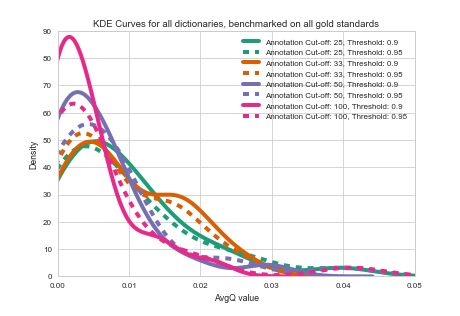
\includegraphics[width=\textwidth]{avgQKDE_method=any.png}
  \captionsetup{width= 0.95\textwidth}
  \caption{\csentence{Kernel density estimates for 30 gold standard datasets.}
      We ran TEA on 30 datasets we believed to be enriched in particulae tissues and pooled all the results to observe the distribution of q-values. The mode of the distribution for dictionaries with annotation cut-offs of 100 and 50 genes are very similar; however, when the cut-off is lowered to 25 genes, the mode of the distribution shifts to the left, potentially signalling a decrease in measurement power.}
	  \label{fig:qvals}
\end{figure}

%pan neuronal
\begin{figure}
  \begin{subfigure}[b]{0.6\textwidth}
    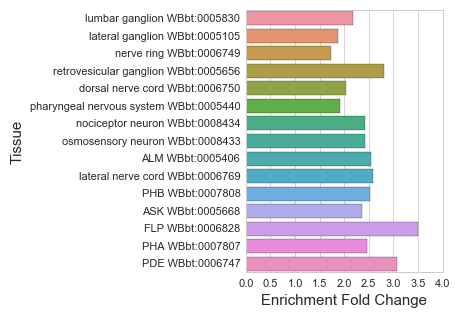
\includegraphics[width=\textwidth]{WBPaper00031532_Larva_Pan_Neuronal_Enriched_WBbt_0003679_1603_33cutoff.png}
    \caption{}
    \label{fig:PanNeuronalWatson33}
  \end{subfigure}
  %
  \begin{subfigure}[b]{0.6\textwidth}
    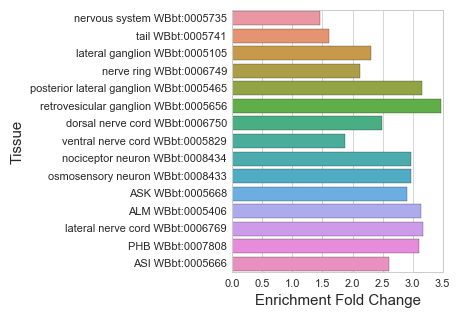
\includegraphics[width=\textwidth]{WBPaper00031532_Larva_Pan_Neuronal_Enriched_WBbt_0003679_1603_50cutoff}
    \caption{}
    \label{fig:PanNeuronalWatson50}
  \end{subfigure}
  \captionsetup{width= 0.95\textwidth}
  \caption{\csentence{Comparison of Enrichment Results for two dictionaries for a pan-neuronal enriched gene set from ~ \cite{Watson2008a}.}
   \textbf{a)} Dictionary with cutoff: 33; threshold: 0.95; method: `any'
   \textbf{b)} Dictionary with cutoff: 50; threshold: 0.95; method: `any'
   }
   \label{fig:interagree}
\end{figure}

%agreements
\begin{figure}
  \begin{subfigure}[b]{0.6\textwidth}
    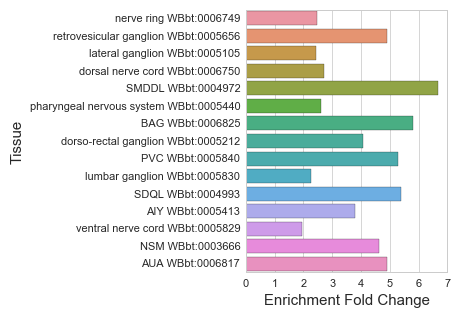
\includegraphics[width=\textwidth]{WBPaper00024970_GABAergic_neuron_specific_WBbt_0005190_247_33cutoff.png}
    \caption{}
    \label{fig:agreement1}
  \end{subfigure}
  %
  \begin{subfigure}[b]{0.6\textwidth} 	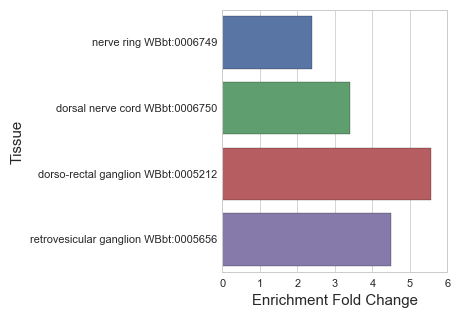
\includegraphics[width=\textwidth]{WBPaper00037950_GABAergic-motor-neurons_larva_enriched_WBbt_0005190_132_33cutoff.png}
    \caption{}
    \label{fig:agreement2}
  \end{subfigure}
  \captionsetup{width= 0.95\textwidth}
  \caption{\csentence{Independently derived genesets show similar results within a given dictionary}
  \textbf{a)} Gene set from  \cite{Watson2008a}. Dictionary with cutoff: 33; threshold: 0.95; method: `any'
  \textbf{b)} Gene set from  \cite{Spencer2011}. Dictionary with cutoff: 50; threshold: 0.95; method: `any'
   }
   \label{fig:intragree}
\end{figure}


%results Figures - engelmann et al reanalysis
%labels are missing.
\begin{figure}[h!]
    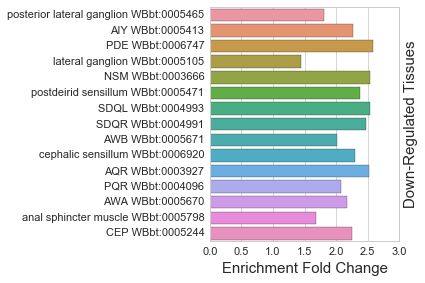
\includegraphics[width=\textwidth]{figures/DrechmeriaconiosporaEnrichment.png}
	\captionsetup{width= 0.95\textwidth}
  	\caption{\csentence{\emph{D. coniospora} enrichment results}
      Genes altered in \emph{C. elegans} after 24hr exposure to \emph{D. coniospora}, a fungus, show enrichment
	  in many neuronal tissues.}
	\label{fig:Dcon}
\end{figure}

\begin{figure}[h!]
    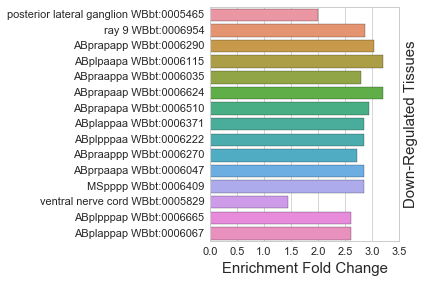
\includegraphics[width=\textwidth]{figures/HarposporiumspEnrichment.png}
	\captionsetup{width= 0.95\textwidth}
	\caption{\csentence{\emph{Harposporium sp.} enrichment results}
      Genes altered in \emph{C. elegans} after 24hr exposure to \emph{Harposporium sp.} a fungus, shows enrichment
	  in the posterior lateral ganglion, similarly to \emph{D. coniospora}. This particular fungus seems to affect
	  genes normally associated with neuronal precursor tissues as well. 
	  }
	\label{fig:Hsp}
\end{figure}

\begin{figure}[h!]
    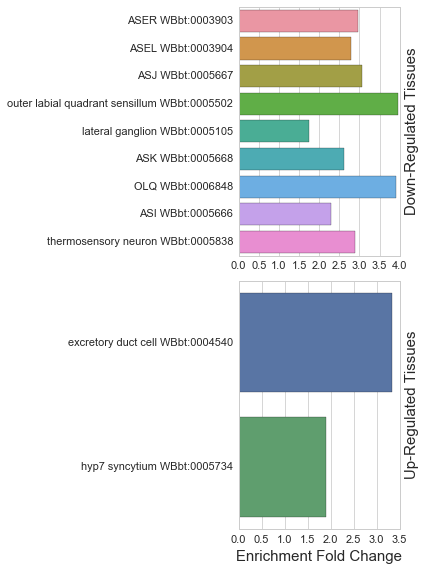
\includegraphics[width=\textwidth]{figures/SerratiamarcescensEnrichment.png}
	\captionsetup{width= 0.95\textwidth}
  	\caption{ \csentence{\emph{Serratia marcescens} enrichment results}
      Genes altered in \emph{C. elegans} after 24hr exposure to \emph{Serratia marcescens}, a bacterium, shows 
	  down-regulation of chemosensory neurons notably ASER, ASEL, ASJ and ASK. The lateral ganglions are also 
	  affected. Up-regulated genes are overrepresented for terms involving the excretory duct cell and hypodermis.
	}  
	\label{fig:Smar}
\end{figure}

\begin{figure}[h!]
    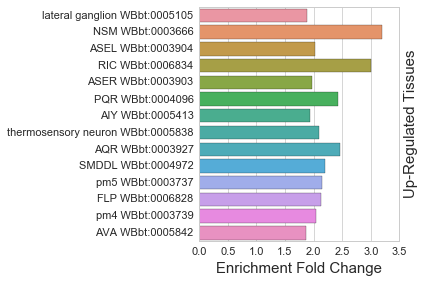
\includegraphics[width=\textwidth]{figures/EnterococcusfaecalisEnrichment.png}
	\captionsetup{width= 0.95\textwidth}
  	\caption{\csentence{\emph{E. faecalis} enrichment results}
      Genes altered in \emph{C. elegans} after 24hr exposure to \emph{E. faecalis}, a bacterium, shows an unusual pattern:
	  No terms were identified as enriched in the down-regulated category. Surprisingly, up-regulated genes show enrichment
	  of various head neurons that were down-regulated with exposure to other pathogens. Interestingly, some pharyngeal
	  muscle terms are also enriched. 
	  }
	\label{fig:Efaec}
\end{figure}

\begin{figure}[h!]
    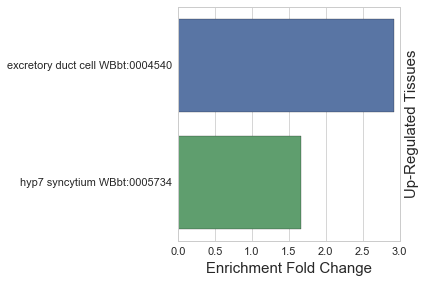
\includegraphics[width=\textwidth]{figures/OtorhabdusluminescensEnrichment.png}
	\captionsetup{width= 0.95\textwidth}
  	\caption{\csentence{\emph{O. luminescens} enrichment results}
      Genes altered in \emph{C. elegans} after 24hr exposure to \emph{O. luminescens}, a bacterium, shows no
	  significantly enriched terms in down-regulated genes. However, up-regulated genes suggest that the hypodermis
	  and excretory duct cell may be affected by infection. 
	  }
	\label{fig:Olum}
\end{figure}

%%%%%%%%%%%%%%%%%%%%%%%%%%%%%%%%%%%
%%                               %%
%% Tables                        %%
%%                               %%
%%%%%%%%%%%%%%%%%%%%%%%%%%%%%%%%%%%

%% Use of \listoftables is discouraged.
%%
\section*{Tables}
\begin{table}[h!]
\caption{Parameter specifications and number of tissues for all dictionaries.}
	\csvautotabular{figures/TissueNumbers.csv}
	\label{tab:DictionarySpecs}
\end{table}

%%%%%%%%%%%%%%%%%%%%%%%%%%%%%%%%%%%
%%                               %%
%% Additional Files              %%
%%                               %%
%%%%%%%%%%%%%%%%%%%%%%%%%%%%%%%%%%%

\section*{Additional Files}
  \subsection*{Additional file 1 --- IPython Notebook}
    Tutorial for users interested in using our software within a python script


\end{backmatter}
\end{document}
